\documentclass[a4paper,10pt]{article}
\usepackage[utf8]{inputenc}
\usepackage{polski}
\usepackage{graphicx}
\usepackage{listings}
\usepackage[usenames,dvipsnames]{color}
\addtolength{\hoffset}{-1cm}
\addtolength{\voffset}{-2cm}
\addtolength{\textwidth}{2cm}
\addtolength{\textheight}{3cm}


\title{Sprawozdanie ISS\newline\small Ćwiczenie 1: Podstawy tworzenia opisów i modelowania obiektów sterowania}

\author{Adam Jordanek 168139, Tomasz Klimek 168092}

\lstset{
    language=Matlab,
    basicstyle=\scriptsize,
    aboveskip={1.5\baselineskip},
    columns=fixed,
    showstringspaces=false,
    extendedchars=true,
    breaklines=true,
    tabsize=4,
    prebreak = \raisebox{0ex}[0ex][0ex]{\ensuremath{\hookleftarrow}},
    frame=single,
    showtabs=false,
    showspaces=false,
    showstringspaces=false,
    identifierstyle=\ttfamily,
    keywordstyle=\color[rgb]{0,0,1},
    commentstyle=\color[rgb]{0.133,0.545,0.133},
    stringstyle=\color[rgb]{0.627,0.126,0.941},
    numbers=left,
    numberstyle=\tiny,
    stepnumber=1,
    numbersep=5pt,
    captionpos=b,
    escapeinside={\%*}{*)}
}



\begin{document}
\maketitle

\section{Wstęp}\label{sec:wstęp}
%TODO skopiowane z listy (trzeba to przerobić)
Tworzenie opisów (modeli) matematycznych obiektów sterowania, a także wykorzystanie tych opisów do badania i analizy (modelowania) obiektów – są istotnymi czynnościami w trakcie projektowania informatycznych systemów sterowania. Do realizacji tych czynności w praktyce inżynierskiej powszechnie stosuje się narzędzie informatyczne Matlab wraz ze specjalistycznym oprogramowaniem dodatkowym (tzw. toolbox’y) oraz nakładką Simulink.

\section{Zadanie 1 \textit{\small Tworzenie modeli matematycznych}}\label{sec:zad1}

\begin{itemize}
\item Inercyjny I rzędu

\begin{itemize}
\item Transmitancja	
	\begin{eqnarray}
		G(s)= {k \over {Ts + 1}} = {Y(s) \over U(s)}
	\end{eqnarray}
\item Równanie różniczkowe
	\begin{eqnarray}
		\nonumber Y(s) = {k \over {Ts + 1}} U(s)\\ 
		\nonumber TsY(s) + Y(s) = kU(s)\\
		T\dot{y}(t) + y(t) = ku(t) \label{eq:iter_rozn}
	\end{eqnarray}
\item Równanie stanu
\newline Ogólna postać równania stanu:
	\begin{eqnarray}
		\nonumber \left\{ \begin{array}{l}
			\dot{x}(t) = Ax(t) + Bu(t)\\
			y(t) = C^{T}x(t)
		\end{array} \right.
	\end{eqnarray}
W równaniu różniczkowym wyjście obiektu jest najwyżej w pierwszej pochodnej, więc mamy do czynienia z obiektem stopnia pierwszego, a wektor stanu x(t) będzie reprezentowany przez jednoelementowy wektor $x(t) = y(t)$, parametry A, B i C będą zwykłymi parametrami liczbowymi, a równanie stanu można zapisać jako:
	\begin{eqnarray}
		\nonumber \left\{ \begin{array}{l}
			\dot{x}(t) = ax(t) + bu(t)\\
			y(t) = cx(t)
		\end{array} \right.
	\end{eqnarray}
Aby uzyskać równanie stanu wystarczy zauważyć, że c=1, oraz przekształcić równanie \ref{eq:iter_rozn} w następujący sposób:
	\begin{eqnarray}
		\nonumber T\dot{y}(t) + y(t) = ku(t)\\
		\nonumber T\dot{x}(t) + x(t) = ku(t)\\
		\nonumber T\dot{x}(t) = - x(t) + u(t)\\
		\dot{x}(t) = -{1 \over T}x(t) + {k \over T}u(t)
	\end{eqnarray}
W ten sposób przyrównując otrzymaliśmy gotowe równanie stanu.
	\begin{eqnarray}
		\left\{ \begin{array}{l}
			\dot{x}(t) = -{1 \over T}x(t) + {k \over T}u(t)\\
			y(t) = x(t)
		\end{array} \right.
	\end{eqnarray}
\item Opis w Matlabie
\newline Opis za pomocą równania stanu w Matlabie uzyskuje się przez podanie współczynników wielomianów $Y(s)$ oraz $U(s)$ z transmitancji (zaczynając od najwyższej) do funkcji $tf2ss(Y, U)$, która zwróci parametry równania stanu.
Ponieważ w Matlabie nie możemy stosować stałych jak k, czy T, podamy w ich miejsce wartości liczbowe.
\newline\newline Dla $k=1$, $T=2$
\newline $>>[A,B,C] = tf2ss([1], [2 \ 1])$
\newline Zwraca wynik:
$A = -0.5, B = 1, C = 0.5$
\newline \newline Parametry zwrócone przez Matlaba różnią się od obliczonych przez nas prawdopodobnie dlatego, że Matlab przyjął inny wektor x(t) na samym początku. Jednak oba opisy są równoważne, ponieważ można przedstawić je w taki sposób:
		\begin{eqnarray}
		\nonumber \left\{ \begin{array}{l}
			\dot{x}(t) = -0.5x(t) + u(t)\\
			y(t) = 0.5x(t)
		\end{array} \right.\\
		\nonumber \dot{y}(t) = 0.5\dot{x}(t)\\
		\nonumber \dot{y}(t) = -0.25x(t) + 0.5u(t)\\
		\nonumber \dot{y}(t) = -0.5y(t) + 0.5u(t)\\
		2\dot{y}(t) + y(t) = u(t)
	\end{eqnarray}
Po porównaniu wyniku przekształceń z równaniem \ref{eq:iter_rozn} widzimy, że $k=1$, $T=2$, czyli tak jak założyliśmy.

\end{itemize}

\item Inercyjny II rzędu
\begin{itemize}
\item Transmitancja
	\begin{eqnarray}
		G(s)= {k \over \left({T_{1}s + 1}\right) \left({T_{2}s + 1}\right)} = {Y(s) \over U(s)}
	\end{eqnarray}
\item Równanie różniczkowe
	\begin{eqnarray}
		\nonumber Y(s) = {k \over {\left({T_{1}s + 1}\right) \left({T_{2}s + 1}\right)}} U(s)\\
		\nonumber Y(s)\left({T_{1}s + 1}\right) \left({T_{2}s + 1}\right)= kU(s)\\
		\nonumber T_{1}T_{2}s^{2}Y(s) + \left({T_{1} + T_{2}}\right) s Y(s) + Y(s)= kU(s)\\
		T_{1}T_{2}\ddot{y}(t) + \left({T_{1} + T_{2}}\right) \dot{y}(t) + y(t)= ku(t) \label{eq:inerc_rozn}
	\end{eqnarray}
\item Równanie stanu
\newline W równaniu różniczkowym wyjście obiektu jest najwyżej w drugiej pochodnej, więc mamy do czynienia z obiektem stopnia drugiego, a wektor stanu x(t) będzie reprezentowany przez dwuelementowy wektor:
 	\begin{eqnarray}
		\nonumber x(t) = \left[ 
			\begin{array}{l}
				x_{1}(t)\\
				x_{2}(t)
			\end{array}
		\right] = \left[ 
			\begin{array}{l}
				y(t)\\
				\dot{y}(t)
			\end{array}
		\right]
	\end{eqnarray}
Parametry A, B i C będą natomiast miały postać:
	\begin{eqnarray}
		\nonumber A = \left[ 
			\begin{array}{ll}
				a_{11} & a_{12}\\
				a_{21} & a_{22}
			\end{array}
		\right], B = \left[ 
			\begin{array}{l}
				b_{1}\\
				b_{2}
			\end{array}
		\right], C = \left[ 
			\begin{array}{l}
				c_{1}\\
				c_{2}
			\end{array}
		\right]
	\end{eqnarray}
Aby uzyskać równanie stanu przekształcamy równanie \ref{eq:inerc_rozn} otrzynując:
	\begin{eqnarray}
		\nonumber T_{1}T_{2}\ddot{y}(t) + \left({T_{1} + T_{2}}\right) \dot{y}(t) + y(t)= ku(t)\\
		\nonumber T_{1}T_{2}\dot{x_{2}}(t) + \left({T_{1} + T_{2}}\right) x_{2}(t) + x_{1}(t)= ku(t)\\
		\nonumber T_{1}T_{2}\dot{x_{2}}(t) = - \left({T_{1} + T_{2}}\right) x_{2}(t) - x_{1}(t) + ku(t)\\
		\dot{x_{2}}(t) = -{{T_{1} + T_{2}} \over T_{1}T_{2}}x_{2}(t) -{1 \over T_{1}T_{2}}x_{1}(1) + {k \over T_{1}T_{2}}u(t)
	\end{eqnarray}
Z otrzymanego równania możemy wywnioskować wartości parametrów A, B i C, oraz zapisać ostateczną postać równania stanu:
	\begin{eqnarray}
		\left\{
			\begin{array}{l}
				x(t) = \left[ 
			\begin{array}{ll}
				0 & 1\\
				-{1 \over T_{1}T_{2}} & -{{T_{1} + T_{2}} \over T_{1}T_{2}}
			\end{array}
		\right] x(t) + \left[ 
			\begin{array}{l}
				0\\
				{k \over T_{1}T_{2}}
			\end{array}
		\right] u(t)\\
				y(t) = \left[ 
			\begin{array}{ll}
				1 & 0
			\end{array}
		\right]x(t)
			\end{array} \right.
	\end{eqnarray}
\item Opis w Matlabie
\newline Opis uzyskamy analogicznie jak w poprzednich przykładach.
\newline\newline Dla $k=1$, $T=2$
\newline $>>[A,B,C] = tf2ss([1], [2 \ 3 \ 1])$
\newline Zwraca wynik:
$A = \left[ \begin{array}{ll} -1.5 & -0.5\\ 1 & 0 \end{array} \right], B = \left[ \begin{array}{l} 1\\ 0 \end{array} \right], C = \left[ \begin{array}{ll} 0 & 0.5 \end{array} \right]$
\newline \newline Parametry zwrócone przez Matlaba różnią się od obliczonych przez nas prawdopodobnie dlatego, że Matlab przyjął inny wektor x(t) na samym początku. Jednak oba opisy są równoważne, ponieważ można przedstawić je w taki sposób:
	\begin{eqnarray}
		\nonumber \left\{ \begin{array}{l}
			\dot{x_{1}}(t) = -1.5x_{1}(t) -0.5x_{2} + u(t)\\
			\dot{x_{2}}(t) = x_{1}\\
			y(t) = 0.5x(t)
		\end{array} \right. \\
		\nonumber \ddot{y}(t) = 0.5\ddot{x_{2}}(t)\\
		\nonumber \ddot{y}(t) = 0.5\dot{x_{1}}(t)\\
		\nonumber \ddot{y}(t) = -0.75x_{1}(t) -0.25x_{2}(t) + 0.5u(t)\\
		\nonumber \ddot{y}(t) = -1,5\dot{y}(t) -0.5y(t) + 0.5u(t)\\
		2\ddot{y}(t) + 3\dot{y}(t) + y(t) = u(t)
	\end{eqnarray}
\end{itemize}
Po porównaniu wyniku przekształceń z równaniem \ref{eq:inerc_rozn} widzimy, że $T_{1}T_{2}=2$, $T_{1} + T_{2}=3$, czyli tak pasuje do założonych.

\item Całkujący rzeczywisty

\begin{itemize}
\item Transmitancja	
	\begin{eqnarray}
		G(s)= {k \over {s \left( Ts + 1 \right) }} = {Y(s) \over U(s)}
	\end{eqnarray}
\item Równanie różniczkowe
	\begin{eqnarray} 
		\nonumber Y(s) = {k \over {s \left( Ts + 1 \right) }} U(s)\\ 
		\nonumber Ts^{2}Y(s) + sY(s) = kU(s)\\
		T\ddot{y}(t) + \dot{y}(t) = ku(t) \label{eq:calk_rozn}
	\end{eqnarray}
\item Równanie stanu
\newline W równaniu różniczkowym wyjście obiektu jest najwyżej w drugiej pochodnej, więc mamy do czynienia z obiektem stopnia drugiego, a wektor stanu x(t) będzie reprezentowany przez dwuelementowy wektor:
 	\begin{eqnarray}
		\nonumber x(t) = \left[ 
			\begin{array}{l}
				x_{1}(t)\\
				x_{2}(t)
			\end{array}
		\right] = \left[ 
			\begin{array}{l}
				y(t)\\
				\dot{y}(t)
			\end{array}
		\right]
	\end{eqnarray}
Parametry A, B i C będą natomiast miały postać:
	\begin{eqnarray}
		\nonumber A = \left[ 
			\begin{array}{ll}
				a_{11} & a_{12}\\
				a_{21} & a_{22}
			\end{array}
		\right], B = \left[ 
			\begin{array}{l}
				b_{1}\\
				b_{2}
			\end{array}
		\right], C = \left[ 
			\begin{array}{l}
				c_{1}\\
				c_{2}
			\end{array}
		\right]
	\end{eqnarray}
Aby uzyskać równanie stanu przekształcamy równanie \ref{eq:calk_rozn} otrzynując:
	\begin{eqnarray}
		\nonumber T\ddot{y}(t) + \dot{y}(t) = ku(t)\\
		\nonumber T\dot{x_{2}}(t) + x_{2}(t) = ku(t)\\
		\nonumber T\dot{x_{2}}(t) = - x_{2}(t) + ku(t)\\
		\dot{x_{2}}(t) = -{1 \over T}x_{2}(t) + {k \over T}u(t)
	\end{eqnarray}
Z otrzymanego równania możemy wywnioskować wartości parametrów A, B i C, oraz zapisać ostateczną postać równania stanu:
	\begin{eqnarray}
		\left\{
			\begin{array}{l}
				x(t) = \left[ 
			\begin{array}{ll}
				0 & 1\\
				0 & -{1 \over T}
			\end{array}
		\right] x(t) + \left[ 
			\begin{array}{l}
				0\\
				{k \over T}
			\end{array}
		\right] u(t)\\
				y(t) = \left[ 
			\begin{array}{ll}
				1 & 0
			\end{array}
		\right]x(t)
			\end{array} \right.
	\end{eqnarray}
\item Opis w Matlabie
\newline Opis uzyskamy analogicznie jak w poprzednich przykładach.
\newline\newline Dla $k=1$, $T=2$
\newline $>>[A,B,C] = tf2ss([1], [2 \ 1 \ 0])$
\newline Zwraca wynik:
$A = \left[ \begin{array}{ll} -0.5 & 0\\ 1 & 0 \end{array} \right], B = \left[ \begin{array}{l} 1\\ 0 \end{array} \right], C = \left[ \begin{array}{ll} 0 & 0.5 \end{array} \right]$
\newline \newline Parametry zwrócone przez Matlaba różnią się od obliczonych przez nas prawdopodobnie dlatego, że Matlab przyjął inny wektor x(t) na samym początku. Jednak oba opisy są równoważne, ponieważ można przedstawić je w taki sposób:
	\begin{eqnarray}
		\nonumber \left\{ \begin{array}{l}
			\dot{x_{1}}(t) = -0.5x_{1}(t) + u(t)\\
			\dot{x_{2}}(t) = x_{1}\\
			y(t) = 0.5x(t)
		\end{array} \right. \\
		\nonumber \ddot{y}(t) = 0.5\ddot{x_{2}}(t)\\
		\nonumber \ddot{y}(t) = 0.5\dot{x_{1}}(t)\\
		\nonumber \ddot{y}(t) = -0.25x_{1}(t) + 0.5u(t)\\
		\nonumber \ddot{y}(t) = -0,5\dot{y}(t) + 0.5u(t)\\
		2\ddot{y}(t) + \dot{y}(t) = u(t)
	\end{eqnarray}
Po porównaniu wyniku przekształceń z równaniem \ref{eq:calk_rozn} widzimy, że $k=1$, $T=2$, czyli tak jak założyliśmy.

\end{itemize}

\item Różniczkujący rzeczywisty
\begin{itemize}
\item Transmitancja
	\begin{eqnarray}
		G(s)= {ks \over \left({Ts + 1}\right)} = {Y(s) \over U(s)}
	\end{eqnarray}
\item Równanie różniczkowe
	\begin{eqnarray}
		\nonumber Y(s) = {ks \over \left({Ts + 1}\right)}  U(s)\\
		\nonumber TsY(s)+Y(s)=k s U(s)\\
		T\dot{y}(t)+y=k\dot{u}(t) \label{eq:rozn_rozn}
	\end{eqnarray}
\item Równanie stanu
\newline W równaniu różniczkowym wyjście obiektu jest najwyżej w pierwszej pochodnej, więc mamy do czynienia z obiektem stopnia pierwszego, jednak ponieważ wejście również jest w pierwszej pochodnej, więc wektor stanu x(t) będzie reprezentowany przez jednoelementowy wektor $x(t) = y(t) + \alpha u(t)$, parametry A, B, C i D będą zwykłymi parametrami liczbowymi, a równanie stanu można zapisać jako:
	\begin{eqnarray}
		\nonumber \left\{ \begin{array}{l}
			\dot{x}(t) = ax(t) + bu(t)\\
			y(t) = cx(t) + du(t)
		\end{array} \right.\\
		\nonumber \left\{ \begin{array}{l}
			\dot{y}(t) + \alpha \dot{u}(t) = ay(t) + a\alpha u(t) + bu(t)\\
			y(t) = cy(t) + c\alpha u(t) + du(t)
		\end{array} \right.\\
	\end{eqnarray}
Aby uzyskać równanie stanu wystarczy zauważyć, że $c=1$, $d = -\alpha$, oraz przekształcić równanie \ref{eq:rozn_rozn} w następujący sposób:
	\begin{eqnarray}
		\nonumber T\dot{y}(t) + y(t) = k\dot{u}(t)\\
		\dot{y}(t) + {1 \over T}y(t) = {k \over T}\dot{u}(t)
	\end{eqnarray}
Z tej postaci możemy już wywnioskować wartości pozostałych parametrów i podać gotowe równanie stanu.
	\begin{eqnarray}
		\left\{ \begin{array}{l}
			\dot{x}(t) = -{1 \over T}x(t) - {k \over T^{2}}u(t)\\
			y(t) = x(t) + {k \over T}u(t)
		\end{array} \right.
	\end{eqnarray}
\item Opis w Matlabie
\newline Opis uzyskamy analogicznie jak w poprzednich przykładach.
\newline\newline Dla $k=1$, $T=2$
\newline $>>[A,B,C,D] = tf2ss([1 \ 0], [2 \ 1])$
\newline Zwraca wynik:
$A = -0.5, B = 1, C = -0.25, D = 0.5$
\newline \newline Parametry zwrócone przez Matlaba różnią się od obliczonych przez nas prawdopodobnie dlatego, że Matlab przyjął inny wektor x(t) na samym początku. Jednak oba opisy są równoważne, ponieważ można przedstawić je w taki sposób:
		\begin{eqnarray}
		\nonumber \left\{ \begin{array}{l}
			\dot{x}(t) = -0.5x(t) + u(t)\\
			y(t) = -0.25x(t) + 0.5u(t)
		\end{array} \right.\\
		\nonumber \dot{y}(t) = -0.25\dot{x}(t) + 0.5\dot{u}(t)\\
		\nonumber \dot{y}(t) = 0.0125x(t) - 0.25u(t) + 0.5\dot{u}(t)\\
		\nonumber \dot{y}(t) = 0.25u(t) - 0.5y(t) - 0.25u(t) + 0.5\dot{u}(t)\\
		2\dot{y}(t) + y(t) = \dot{u}(t)
	\end{eqnarray}
Po porównaniu wyniku przekształceń z równaniem \ref{eq:rozn_rozn} widzimy, że $k=1$, $T=2$, czyli tak jak założyliśmy.

\end{itemize}

\item Proporcjonalny
\begin{itemize}
\item Transmitancja	
	\begin{eqnarray}
		G(s)= {k}= {Y(s) \over U(s)}
	\end{eqnarray}
\item Równanie różniczkowe
	\begin{eqnarray} 
		\nonumber Y(s) = k U(s)\\ \label{eq:prop_rozn}
		y(t)= ku(t)
	\end{eqnarray}
\item Równanie stanu
	Nie ma opisu w przestrzeni stanów.
\end{itemize}

\end{itemize}

\section{Zadanie 2 \textit{\small Wyznaczanie charakterystyk czasowych}}\label{sec:zad2}

\begin{itemize}
\item Przy użyciu funkcji impulse(...) i step(...) w programie Matlab
\begin{itemize}
\item Inercyjny I rzędu
\newline 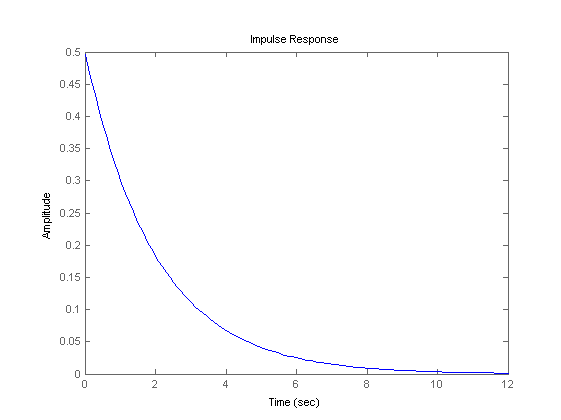
\includegraphics[scale=0.9]{CW1-inercyjny1-impuls}\newline Charakterystyka impulsowa
\newline 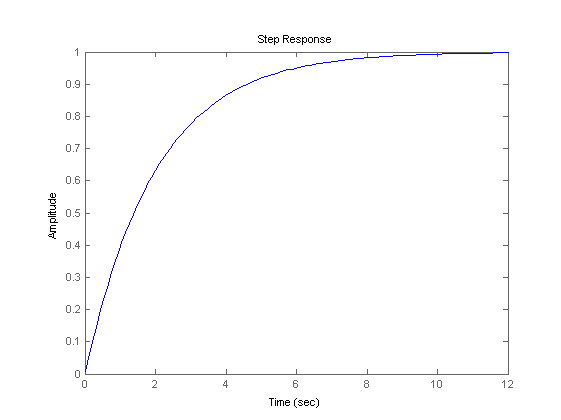
\includegraphics[scale=0.9]{CW1-inercyjny1-skok}\newline Charakterystyka skokowa
\newpage
\item Inercyjny II rzędu 
\newline 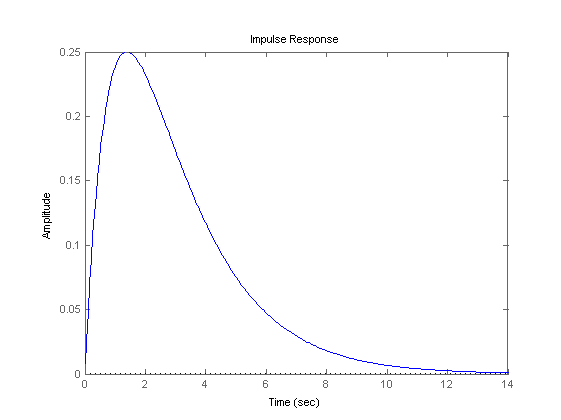
\includegraphics[scale=0.9]{CW1-inercyjny2-impuls}\newline Charakterystyka impulsowa
\newline 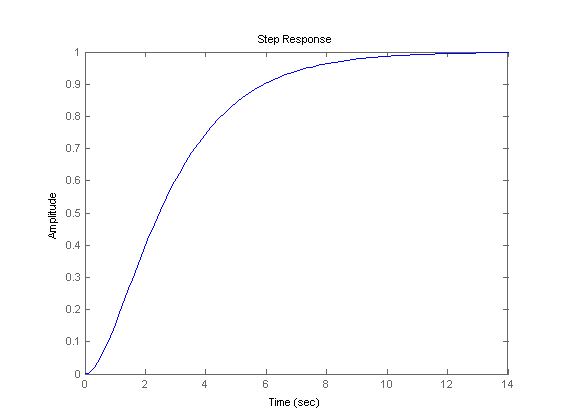
\includegraphics[scale=0.9]{CW1-inercyjny2-skok}\newline Charakterystyka skokowa  
\newpage
\item Całkujący rzeczywisty 
\newline 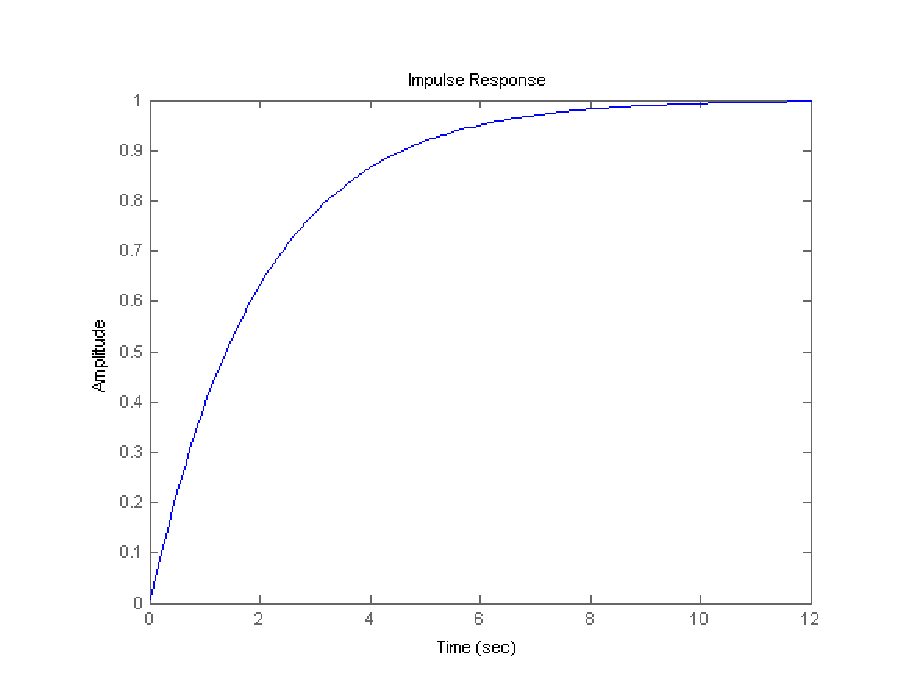
\includegraphics[scale=0.9]{CW1-calkujacy-impuls.eps}\newline Charakterystyka impulsowa
\newline 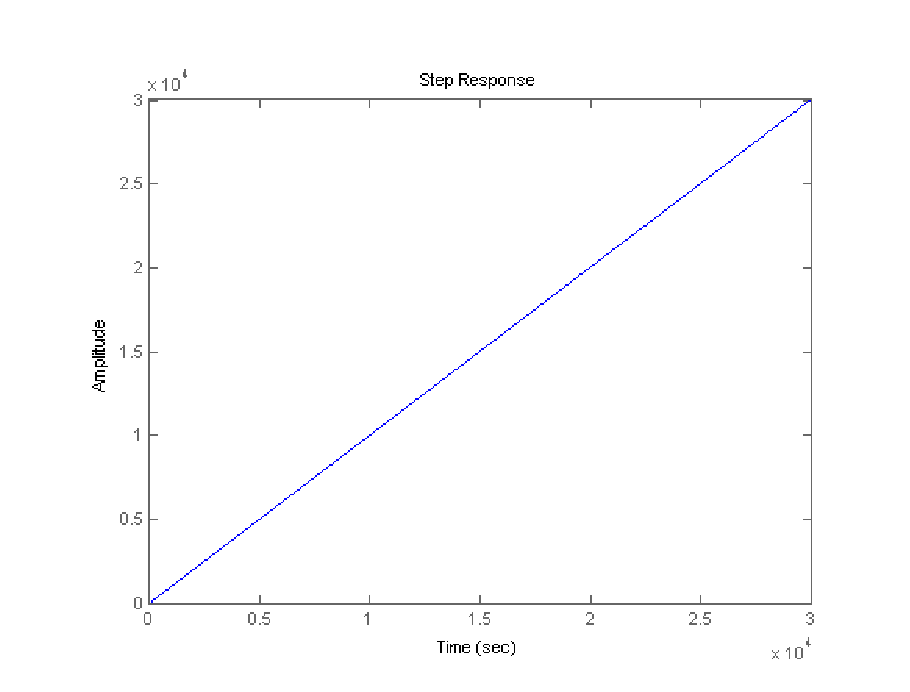
\includegraphics[scale=0.9]{CW1-calkujacy-skok}\newline Charakterystyka skokowa  
\newpage
\item Różniczkujący rzeczywisty 
\newline 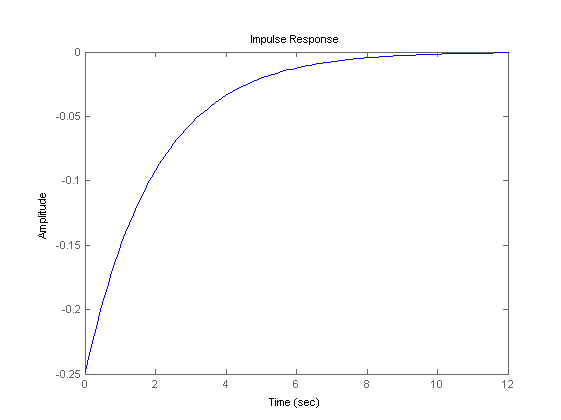
\includegraphics[scale=0.9]{CW1-rozniczkujacy-impuls}\newline Charakterystyka impulsowa
\newline 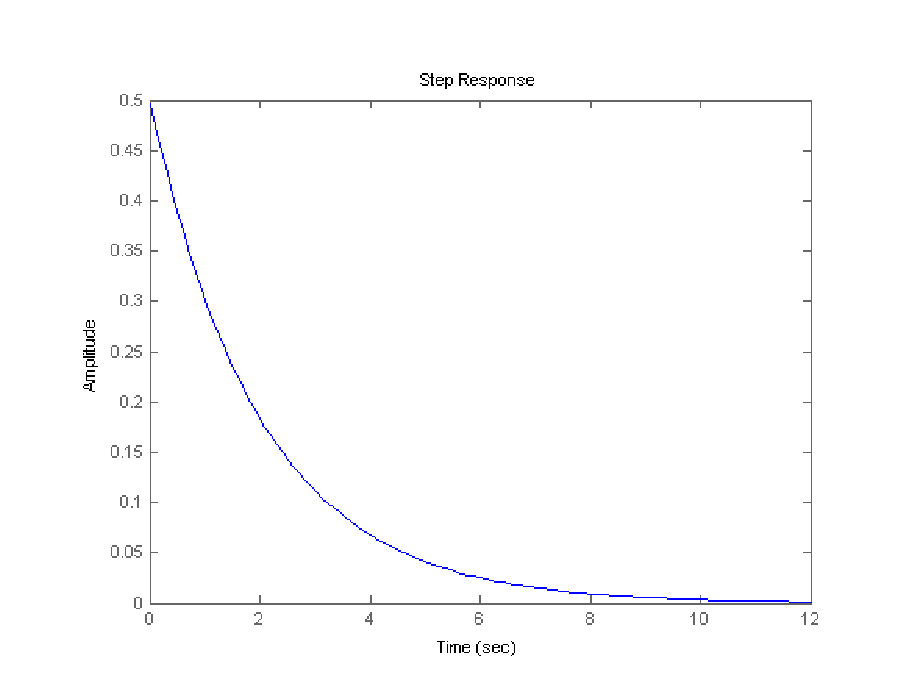
\includegraphics[scale=0.9]{CW1-rozniczkujacy-skok}\newline Charakterystyka skokowa  
\newpage
\item Proporcjonalny 
\newline 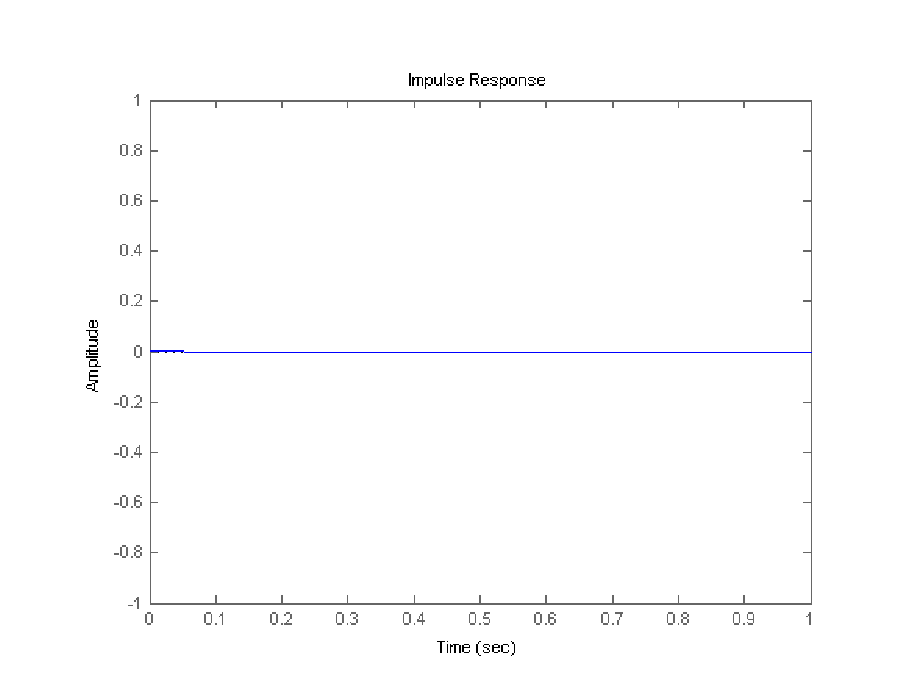
\includegraphics[scale=0.9]{CW1-proporcjonalny-impuls}\newline Charakterystyka impulsowa
\newline 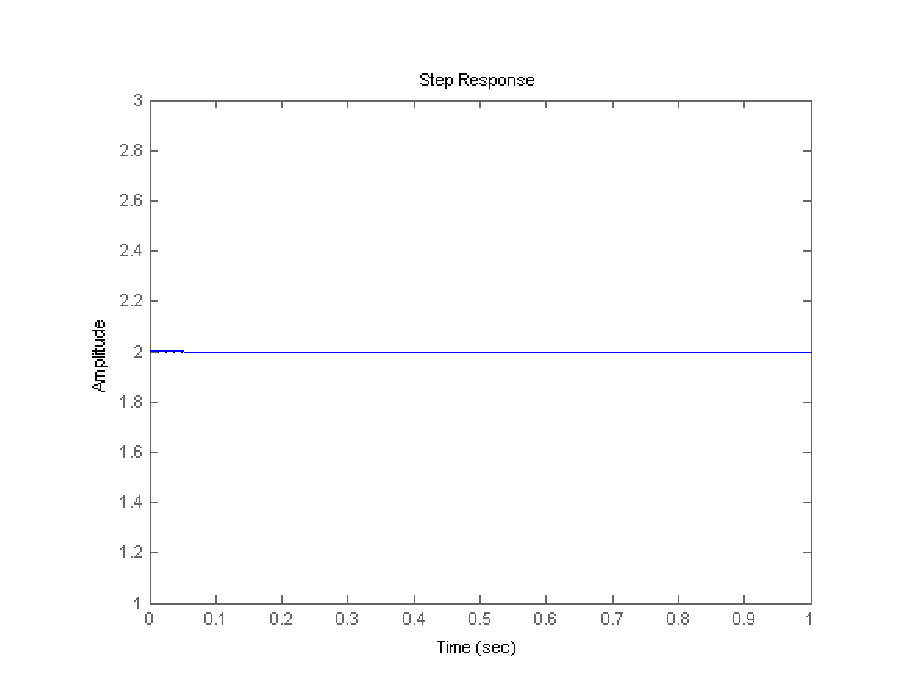
\includegraphics[scale=0.9]{CW1-proporcjonalny-skok}\newline Charakterystyka skokowa  
\end{itemize}

\item Przy użyciu własnych funkcji mImpulse(...) i mStep(...)

	\begin{eqnarray} 
		\dot{x}(t=n \Delta t ) = {x_{n+1}-x_{n} \over {\Delta t}}
	\end{eqnarray}
	\begin{eqnarray} 
		x_{n}=x(t=n \Delta t)
	\end{eqnarray}
	\begin{eqnarray} 
		u_{n}=u(t=n \Delta t)
	\end{eqnarray}
	\begin{eqnarray} 
		y_{n}=y(t=n \Delta t)
	\end{eqnarray}\\
	Dodatkowo korzystamy z:\\
	\begin{eqnarray} 
		\nonumber \dot{x}_{n}=Ax_{n}+Bu_{n}
		\nonumber y_{n}=Cx_{n}
	\end{eqnarray}\\
	Otrzymujemy układ dyskretny:\\
	\begin{eqnarray} 
		\nonumber {x}_{n+1}=(Ax_{n}+Bu_{n}) \Delta t +x_{n}
		\nonumber y_{n}=Cx_{n}
	\end{eqnarray}\\
	Taki układ można już zastosować do napisania funkcji:
\begin{lstlisting}[caption=funkcja mImpulse.m]
function p=mImpulse(A,B,C,D,dt,n)
	y = zeros(1,n);
	x = zeros(size(A),n);
	x(1,1)=1;
	t = 0:dt:dt*(n-1);
	u=1;
	for i=1:n
		y(1,i) = C*x(:,i) + D*u;
		x(:,i+1) = (A*x(:,i)+B*u)*dt + x(:,i);
		u = 0;
	end
	p=plot(t,y(1,:))
end
\end{lstlisting}
Nasz funkcja tworzy wykres charakterystyki impulsowej na podstawie parametrów A,B,C i D będących parametrami rówania stanu (obliczonymi w poprzednim zadaniu) oraz długość kroku i ich ilość. Po pierwszej iteracji u jest zamienione z 1 na 0 tak aby zasymulować impuls.

\begin{lstlisting}[caption=funkcja mStep.m]
function p=mStep(A,B,C,D,dt,n)
	y = zeros(1,n);
	x = zeros(size(A),n);
	t = 0:dt:dt*(n-1);
	u=1;
	for i=1:n
		y(1,i) = C*x(:,i) + D*u;
		x(:,i+1) = (A*x(:,i)+B*u)*dt + x(:,i);
	end
	p=plot(t,y(1,:))
end
\end{lstlisting}
Nasz funkcja tworzy wykres charakterystyki skokowej na podstawie parametrów A,B,C i D będących parametrami rówania stanu (obliczonymi w poprzednim zadaniu) oraz długość kroku i ich ilość. Wartość u jest zawsze równa 1 symulując funkcję jednostkową.

\newpage 
\begin{itemize}
\item Inercyjny I rzędu
\newline 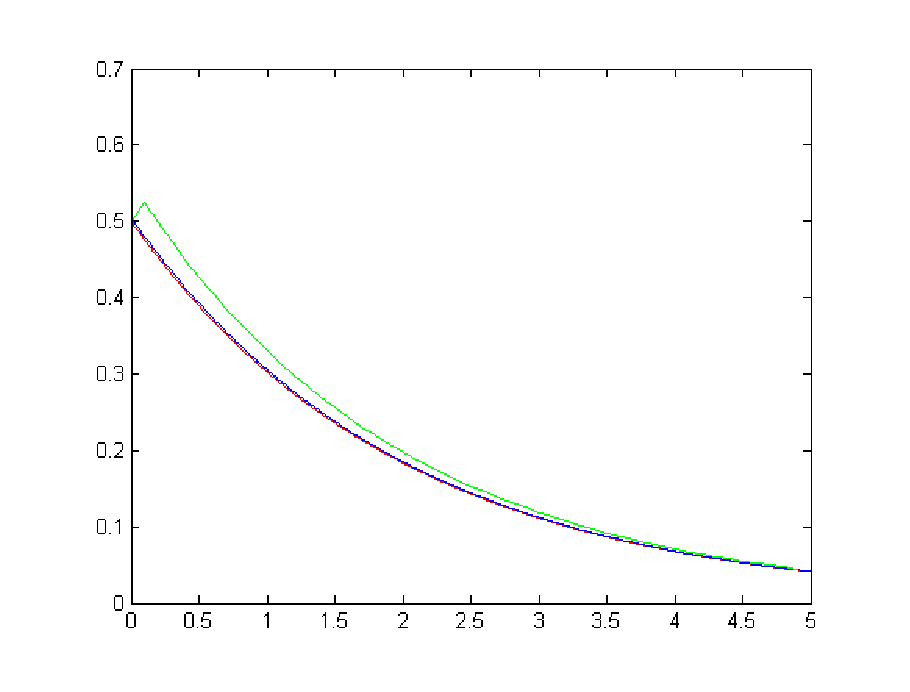
\includegraphics[scale=0.9]{CW1-inercyjny1-mimpuls.eps}\newline Charakterystyka impulsowa
\newline 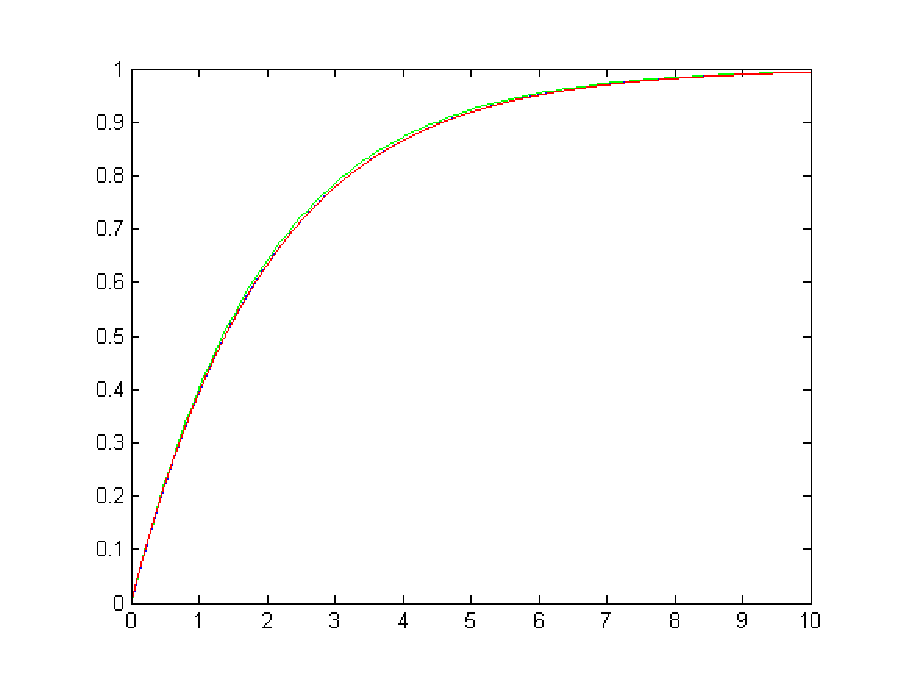
\includegraphics[scale=0.9]{CW1-inercyjny1-mskok.eps}\newline Charakterystyka skokowa
\newpage  
\item Inercyjny II rzędu
\newline 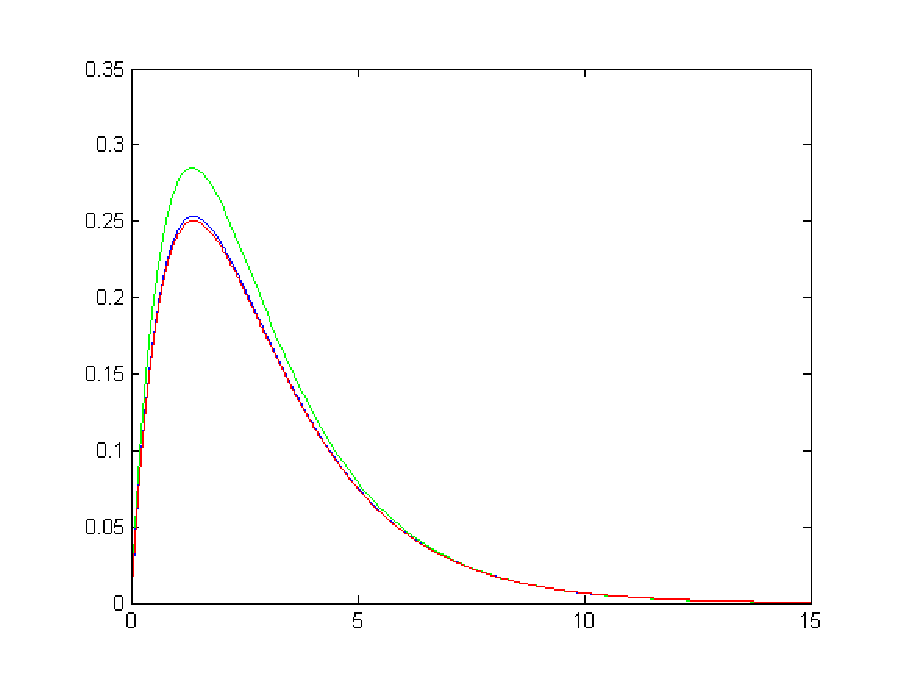
\includegraphics[scale=0.9]{CW1-inercyjny2-mimpuls.eps}\newline Charakterystyka impulsowa
\newline 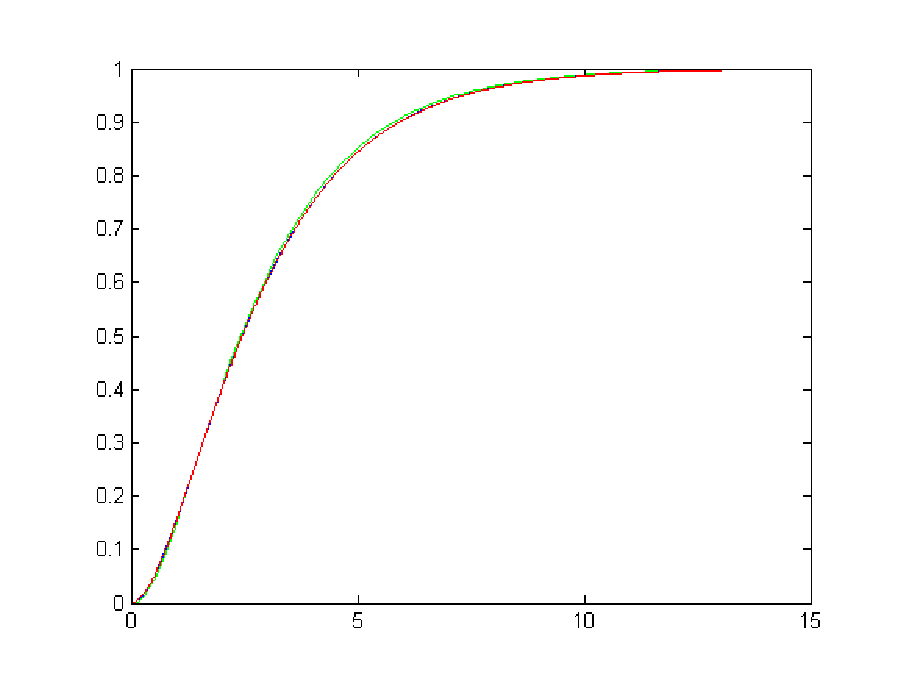
\includegraphics[scale=0.9]{CW1-inercyjny2-mskok.eps}\newline Charakterystyka skokowa
\newpage
\item Całkujący rzeczywisty
\newline 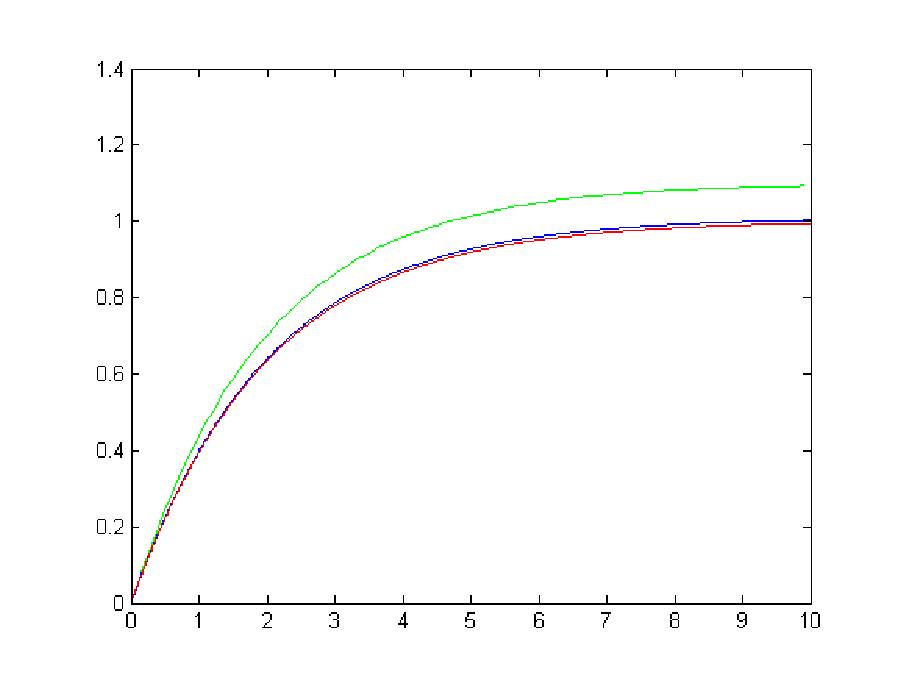
\includegraphics[scale=0.9]{CW1-calkujacy-mimpuls.eps}\newline Charakterystyka impulsowa
\newline 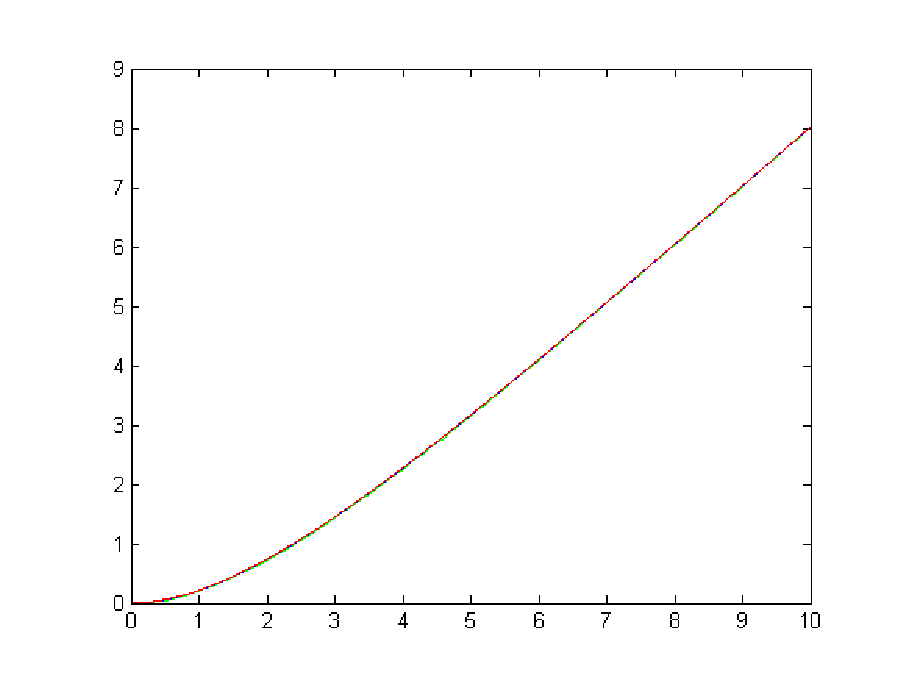
\includegraphics[scale=0.9]{CW1-calkujacy-mskok.eps}\newline Charakterystyka skokowa
\newpage
\item Różniczkujący rzeczywisty
\newline 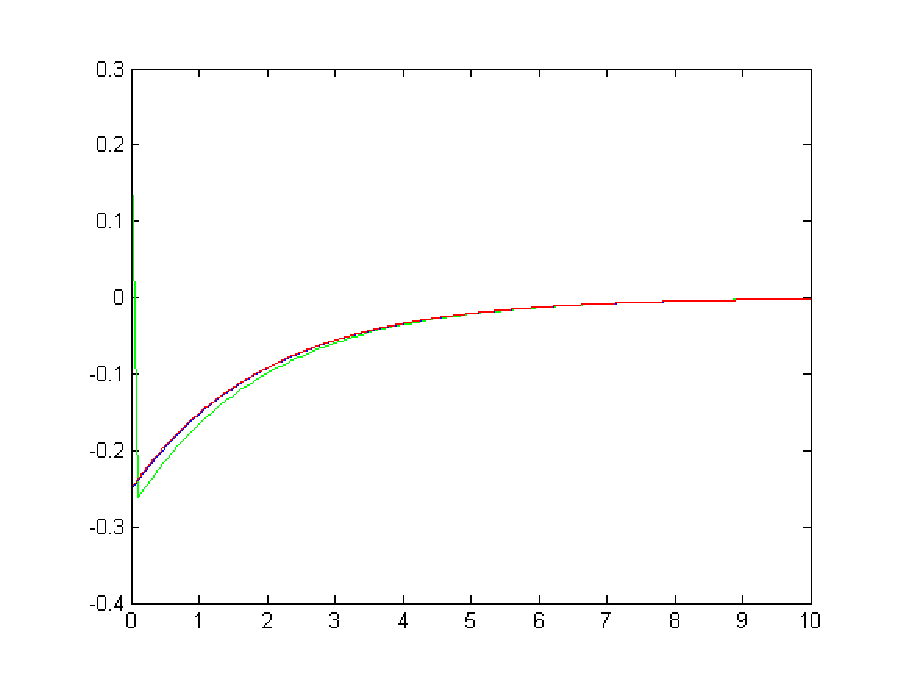
\includegraphics[scale=0.9]{CW1-rozniczkujacy-mimpuls.eps}\newline Charakterystyka impulsowa
\newline 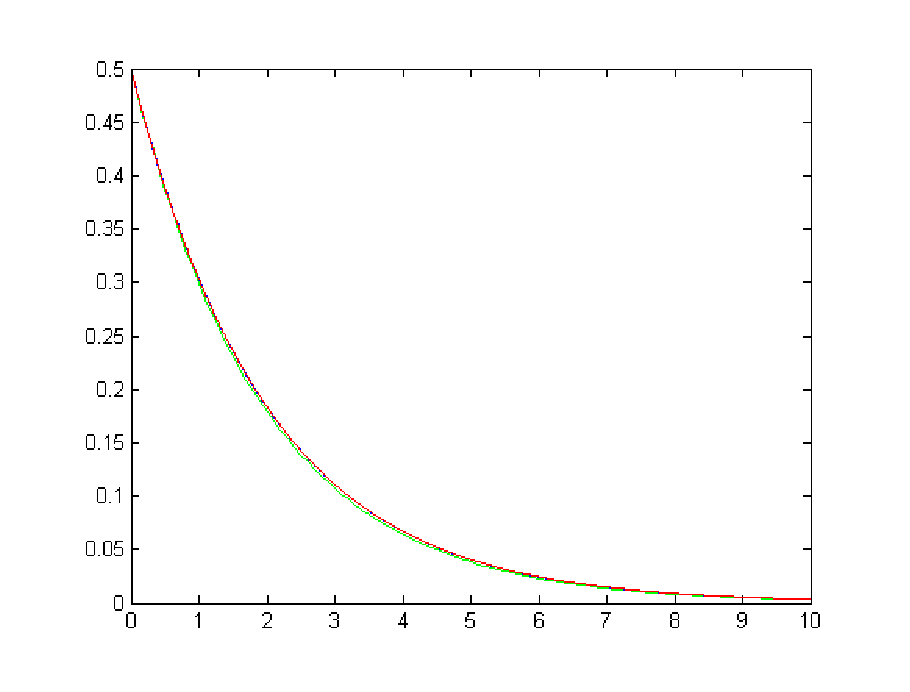
\includegraphics[scale=0.9]{CW1-rozniczkujacy-mskok.eps}\newline Charakterystyka skokowa
\newpage
\item Proporcjonalny 
\newline 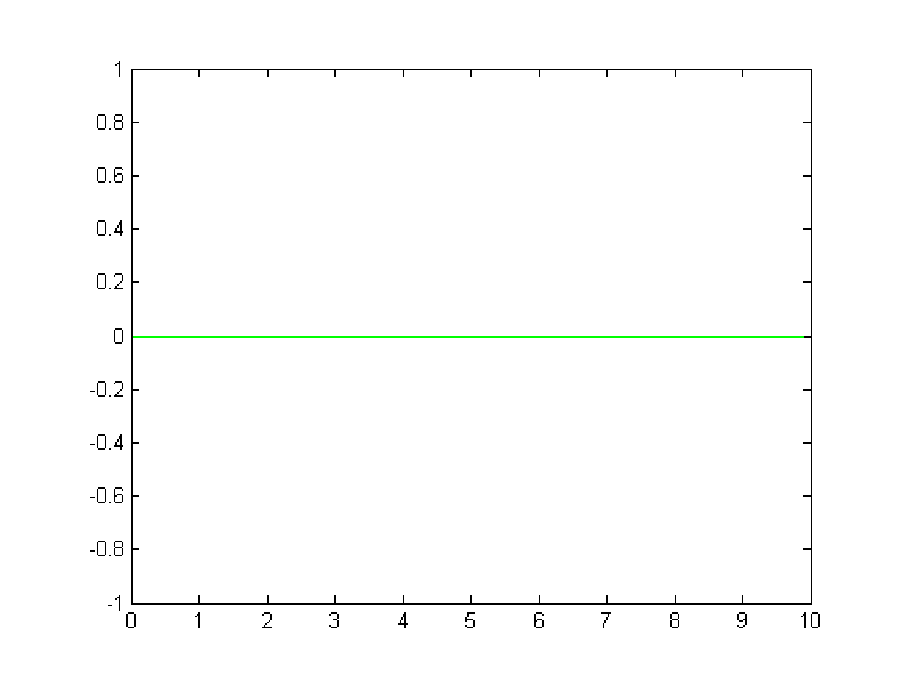
\includegraphics[scale=0.9]{CW1-proporcjonalny-mimpuls.eps}\newline Charakterystyka impulsowa
\newline 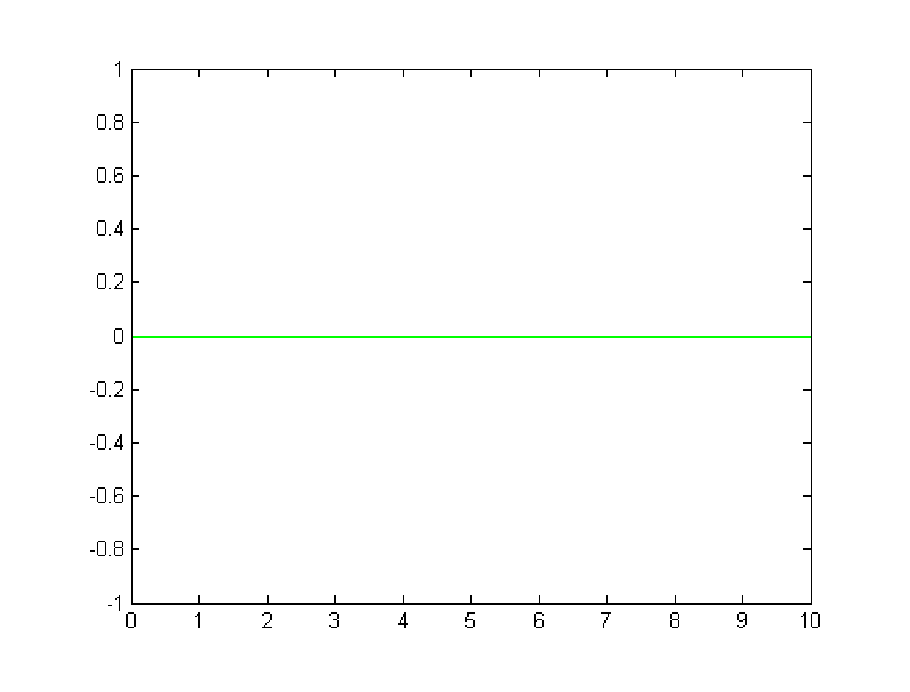
\includegraphics[scale=0.9]{CW1-proporcjonalny-mskok.eps}\newline Charakterystyka skokowa
  
\end{itemize}
\end{itemize}

\section{Zadanie 3 \textit{\small Wyznaczanie parametrów członów dynamicznych}}\label{sec:zad3}

Przepisane dla inercyjnego:
	\begin{eqnarray} 
		g(t)={k \over T} e^{-{t \over T}}
	\end{eqnarray}\\
	
Aby odczytać wartość k i T postępujemy w następujący sposób:
Wyliczamy dla punktu t=0:

	\begin{eqnarray} 
		g(0)={k \over T}
	\end{eqnarray}\\
	Liczymy pochodną:
	\begin{eqnarray} 
		\dot{g}(t)=-{k \over T^{2}} e^{-{t \over T}}
	\end{eqnarray}\\
	Obliczamy wartość pochodnej w punkcjie t=0
	\begin{eqnarray} 
		\dot{g}(0)=-{k \over T^{2}}=-{1 \over T^{2}}g(0)
	\end{eqnarray}\\
Przedstawiamy pochodną dla t=0 jako współczynnik kierunkowy stycznej (s(t)). Załóżmy, że dla t’
dana styczna osiąga wartość 0 (przecina oś Ot). Wartość tego współczynnika ma wartość (wiemy
także, że s(0)=g(0)):
	\begin{eqnarray} 
		{s(t_{2})- s(t_{1}) \over {t_{2} -t_{1}}}={s(t')- s(0) \over {t' -0}}={s(0) \over t'}={g(0) \over t'}
	\end{eqnarray}\\
	Podstawiając:
	\begin{eqnarray} 
		-{g(0) \over t'}= - {1 \over T} g(0)
	\end{eqnarray}\\
	Wychodzi:
	\begin{eqnarray} 
		T=t'
	\end{eqnarray}\\
Interpretacja: wartość parametru T odczytujemy jako argument przecięcia się interpolowanej stycznej
w punkcie t=0 z osią Ot. Mając T wyliczamy k ze wzoru: 
	\begin{eqnarray} 
		k = g (0)T
	\end{eqnarray}
	%Wykres itp
	
	Charakterystyka skokowa:
	\begin{eqnarray} 
			h(t)= k(1- e^{-{1 \over T}})
	\end{eqnarray}		
Aby odczytać wartość k i T postępujemy w następujący sposób:
Bierzemy granicę wartości funkcji
	\begin{eqnarray} 
		\lim_{t \to \infty}{h(t)} = \lim_{t \to \infty}{k(1-e^{-{t \over T}})} 
	\end{eqnarray}	
A więc wartość k odpowiada równaniu asymptoty poziomej w nieskończoności y(t)=k
Aby obliczyć T obliczamy pochodną h(t)
	\begin{eqnarray} 
		\dot{h}(t)={k \over T}e^{-{t \over T}}
	\end{eqnarray}	

\section{Wnioski}\label{sec:wnioski}

1. parametry opisu stanu mogą być różne, a dalej równoznaczne
2. 


\end{document}